
\pagestyle{fancy} \frenchspacing
\lhead{StageControl - automatisierte Steuerung von Ton- und Lichtanlagen (2024/2025)}
\lfoot{Name 1}
\renewcommand{\chaptermark}[1]{\markboth{#1}{}}

\renewcommand{\textfraction}{0}
\renewcommand{\floatpagefraction}{0.999}
\renewcommand{\topfraction}{0.7}
\renewcommand{\bottomfraction}{0.999}

\chapter{Grundlagen und Methoden}

\section{Etablierte Lösungsansätze}
Das Kapitel listet etablierte Lösungsansätze zur Standortermittlung einer Person auf einer Bühne und erklärt diese genauer. Ebenso wie Vor- und Nachteile anhand eines Beispieles.

\subsection{Ausgangsituation des Praxisbeispiels}

Man befindet sich auf der Bühne in der Stadthalle in Ybbs. Folgende Informationen sind wichtig.
\begin{itemize}
	\item \textbf{Gerät zur Standortermittlung: } Android Smartphone
	\item \textbf{Koordinaten der Position: } TBD  
\end{itemize}

\subsection{Manuelle Steuerung}
Eine Person steht auf der Bühne der XY. Eine Möglichkeit die Steuerung der Ton- und Lichtanlagen ist diese für das Event vorher zu programmieren oder manuell während der Show zu steuern. Nun fragt sich die Person: "Wie kann ich diese Ton- und Lichtanlagen steuern?" Die Antworten folgen:

\begin{itemize}
	\item "Manuelle Steuerung der Tonanlage"
	\item "Vorprogrammierung der Lichtanlage"
\end{itemize}

An den erlangten Antworten, kann man erkennen, dass es noch keine automatisierte Lösung für das Problem gibt. Die Genauigkeit der Standortermittlung, die für die automatisierte Steuerung der Anlagen notwendig ist, kann in folgenden Stufen eingeteilt werden: 

\begin{itemize}
	\item \textbf{Stufe 1: }Standort auf Bühne eingeschränkt
	\item \textbf{Stufe 2: }Standort auf Länge und Breite der Bühne eingeschränkt
	\item \textbf{Stufe 3: }Standort auf bestimmten Punkt auf vorhin genannter Bühne eingeschränkt
\end{itemize}

\section{Hardware im Zusammenhang mit StageControl}
Im Fall von StageControl versteht man unter Hardware nicht nur Computerkomponenten, sondern auch hergestellte Konstruktionen, die das Funktionieren der Software bzw. der angesteuerten Komponenten erst möglich machen.

\subsection{Möglichkeiten der Hardwareproduktion}
Die Hardwareproduktion umfasst die Herstellung physischer Komponenten aus unterschiedlichsten Materialien wie z. B. PLA (Polylactide, ein Kunststoff) oder Metallen. Diese Stoffe werden von Unternehmen eingesetzt, die sich mit der Herstellung von Hardware bzw. Prototypen befassen. Dabei gibt es verschiedenste Möglichkeiten und Herangehensweisen in der Hardwareproduktion: 3D-Druck, Laser-Cutting, CNC-Fräsen und die Verwendung von Baukästen wie LEGO®. Im folgenden Abschnitt wird genauer auf die Einsetzbarkeit/Verfügbarkeit, die Vor- und Nachteile zweier Produktionsarten, nämlich 3D-Druck und  für StageControl eingegangen.

\section{3D-Druck}
\subsection{Wie funktioniert 3D-Druck}
Beim 3D-Druck handelt es sich um ein Verfahren, das Schicht für Schicht Material aufträgt, um ein dreidimensionales Objekt zu erschaffen. Diese Art der Produktion wird auch als „Additive Fertigung“ bezeichnet, im Gegensatz zum CNC-Fräsen, das als „subtraktive Fertigung“ bekannt ist.

\subsection{Vorteile des 3D-Drucks}
3D-Druck bietet viele Vorteile für Privatkunden und Unternehmen. Die nachfolgenden Vorteile zählen zu den wichtigsten:
\begin{itemize}
	\item Möglichkeit, komplexe Objekte relativ schnell herzustellen.
	\item Keine Vorlaufzeit nötig, d.h. keine Werkzeugproduktion erforderlich.
	\item Rapid Prototyping \emph{(deutsch „schnelle Prototypenherstellung“)}
	\item Kostengünstige Produktion
	\item Herstellung induvidueller Objekte
\end{itemize} \cite{3D-Druck-Vorteile}

\subsection{Technische Voraussetzungen}
Um den 3D-Druck technisch durchführen zu können, werden folgende Komponenten benötigt:
\begin{itemize} 
	\item 3D-Drucker, bei der durchführung dieser Diplomarbeit stehen uns diese 2 Modelle zur Verfügung: Bambu Lab X1-Carbon  und \emph{Ultimaker 2 Extended+}
	\item 3D-Modellierungsprogramm
	\item 3D-Druck Material (Filament)
	\item Computer
\end{itemize}
Auf den nächsten Seiten wird auf diese Punkte näher eingegangen und ein Vergleich erstellt um die Vor- und Nachteile der genannten 3D-Drucker zu veranschaulichen. \cite{3ds}


\subsection{Druckverfahren}

Um Hardware mittels 3D-Drucks zu erstellen, gibt es verschiedene Möglichkeiten, das Ausgangsmaterial in die gewünschte Form zu bringen. Die gängigsten und weitverbreitesten Verfahren im Überblick: 

\begin{itemize}
	\item \textbf{FFF:} (Fused Filament Fabrication) oder \textbf{FDM} (Fused Deposition Modelling): Hierbei wird Kunststofffilament \emph{(eine einzelne Faser beliebig lang)} verwendet und Schicht für Schicht aufgetragen.
	\item \textbf{SLA:} Diese Technologie verwendet lichtempfindliches Kunstharz, das sich verfestigt. Wird ebenfalls Schicht für Schicht aufgetragen.
	\item \textbf{PBF:} Eine Möglichkeit, diese pulverbasierte Technologie zu nutzen, ist, das Pulver mittels Laser miteinander zu verschmelzen. \cite{kaffka} \cite{3ds}
\end{itemize}

\subsection{Werkstoffe}
3D-Drucker benötigen zum Drucken eines Objektes Material, das sie verbrauchen können, um das Objekt herzustellen. Im Rahmen dieser Diploarbeit werden 2 Werkstoffe ganuer analysiert, nämlich Nylon und Kohlefaser.

\subsubsection{Nylon}
Nylon \emph{(techn. Polyamid)} ist ein langlebiges Material, das sich vorallem durch seine Widerstandfähigkeit gegen Hitze und mechanischen Auseneinwirkungen auszeichnet. Nylon gibt es in unterschiedlichen Ausführung zb. als Filament, Draht oder Pulver mit unterschiedlcihen eigenschaften. \cite{Nylon}
\subsubsection{Kohlefaser}
Kohlefasern wird in Grundpolymeren wie PLA oder Nylon eingearbeitet um eine höhere Stabilität und Resistenz zu erzeugen wie zb. Nylon verstärkt mit Kohlefasern. \cite{Kohlefasern}


\subsection{3D-Drucker}

\subsection{Vergleich der 3D-Drucker}
Wie in der Einleitung des Kapitels \emph{"Hardware im Zusammenhang mit StageControl"} beschrieben, ist eine Möglichkeit zur Herstellung der benötigten Hardware das Drucken mittels eines 3D-Druckers. Um die bereits erwähnten 3D-Drucker (\emph{Bambu Lab X1-Carbon, Ultimaker 2 Extended+}) miteinander zu vergleichen, werden folgende Kriterien herangezogen: die Verarbeitbarkeit des Ausgangsmaterials und die Druckgeschwindigkeit bei einem Düsendurchmesser von 0,4 mm. 

Als Ausgangsmaterial wird bei beiden 3D-Druckern kohlefaserverstärktes Nylon-Filament verwendet.

\begin{table} [H]
	\begin{tabular}{ |p{2cm} |p{5cm}|p{5cm}| }
		\hline
		 \textbf{Kriterien} & \textbf{Ultimaker 2 Extended+}& \textbf{Bambu Lab X1-Carbon 3 Pro}\\
		\hline
		\textbf{Material} & Material kann verarbeitet werden & Materiel kann verarbeitet werden   \\ 
		\textbf{Drucktempo} & Druckt mit einer Geschwindigkeit von 16mm\textsuperscript{3}/s & Druckt mit einer Geschwindigkeit von 32mm\textsuperscript{3}/s   \\  
		\hline
	\end{tabular}
	\caption{Vergleich  Ultimaker 2 Extended+ und Bambu Lab X1-Carbon 3 Pro}
\end{table}

\subsection{Slicer}
\subsubsection{Was ist ein Slicer?}
Ein Slicer ist ein Stück Software, die es erst möglich macht 3D-Modelle auszudrucken, indem es sogenannten G-Code erstellt. G-Code ist die Programmiersprache die von Computern verwendet wird um mit Maschinen zu kommunizieren, wenn die Maschine Bewegungnen ausführen soll. 
\cite{Slicer_G-Code}

\section{3D-Modellierungsprogramme}
Auf dem Markt rund um 3D-Modellierungsprogramme gibt es eine große Auswahl an den verschiedensten Programmen. Von dem anfängerfreundlichen Tinkercad, das durch seine einfache Bedienbarkeit und zahlreiche Tutorials überzeugt, bis hin zu einem der führenden CAD-Programme wie Catia, das in der Industrie für seine leistungsstarken und umfangreichen Funktionen geschätzt wird, ist alles dabei. Im Rahmen dieser Diplomarbeit wurden einige der Marktführer recherchiert und miteinander verglichen.
\cite{CAD-Programme}, \cite{3D-Printing-Software}

\subsection{Vergleich verschiedener 3D-Modellierungsprogramme}

\subsubsection{Autodesk Fusion}
Es eröffnet zahlreiche Anwendungsmöglichkeiten, die von der Prototypenerstellung bis hin zur Entwicklung von Konsumgütern reichen. Dieses Programm bietet umfangreiche Werkzeuge für Design, Engineering und Fertigung. Zudem wird Fusion 360 von vielen internationalen und nationalen Unternehmen verwendet, weil es vielseitig einsetzbar ist und sowohl in kleinen als auch in großen Projekten hervorragende Unterstützung bietet. Dank seiner cloudbasierten Plattform ermöglicht Fusion 360 eine nahtlose Zusammenarbeit und den einfachen Austausch von Projektdaten, was es zu einer bevorzugten Wahl in der modernen Produktentwicklung macht. 
\cite{AutodeskFusion}

\textbf{Vorteile}
\begin{itemize}
	\item Genutzt von vielen Namhaften Unternehmen wie zb. Yamaha oder Panasonic
	\item Große Community
	\item Kostenlose Version für Schulen
\end{itemize} 

\textbf{Nachteile}
\begin{itemize}
	\item Cloud Based; Kann zu Problemen führen, wenn offline genutzt 
	\item Benötigt eine schnelle Internetverbindung
	\item Hoher Anspruch an die Hardware des Computers
	\end{itemize}
 \cite{AutodeskFusionReviews}


\subsubsection{Blender} 
Blender bietet vielseitige Anwendungsmöglichkeiten, von 3D-Modellierung und Animation bis hin zur Spieleentwicklung und visuellen Effekten. Dieses Open-Source-Programm bietet umfassende Werkzeuge für Modellierung, Simulation, Rendering, Compositing und Motion Tracking. Zudem wird Blender von vielen internationalen und nationalen Unternehmen sowie unabhängigen Kunden verwendet, weil es viele Einsatzmöglichkeiten bietet und Gratis zugänglich für jeden ist. Dank seiner aktiven Community und regelmäßigen Updates bleibt Blender immer auf dem neuesten Stand der Technik. 
\cite{Blender}

\textbf{Vorteile}
\begin{itemize}
	\item Gratis 
	\item Open Source Software
	\item Funktioniert auf allen gängigen Betriebssystemen
	\item Regelmäßige Updates
	\item große Community
\end{itemize}

\textbf{Nachteile}
\begin{itemize}
	\item Kein Industriestandard - wird nicht von großen Unternehmen genutzt
	\item Nicht die Benutzerfreundlichste Oberfläche
\end{itemize}
\cite{BlenderPros&Cons}


\subsubsection{FreeCAD}
FreeCAD hat vielseitige Anwendungsmöglichkeiten, von der 3D-Modellierung bis hin zur Erstellung technischer Zeichnungen und Simulationen. Diese Open-Source-Software bietet umfassende Werkzeuge für Ingenieure, Architekten, Produktdesigner und Privatkunden. Zudem wird FreeCAD von vielen Unternehmen sowie unabhängigen Entwicklern genutzt, weil es flexible Einsatzmöglichkeiten bietet. Durch seine modulare Architektur und der aktiven Community wird FreeCAD kontinuierlich weiterentwickelt und verbessert.
 \cite{FreeCAD}  \cite{FreeCAD_2}

\textbf{Vorteile}
\begin{itemize}
	\item Open Source Software
	\item Gratis
	\item Funktionsfähig für alle gängigen Betriebssysteme
	\item Aktive Community	 
\end{itemize}

\textbf{Nachteile}
\begin{itemize}
	\item weniger Nutzer als die bereits genannten Programme
	\item kein Industriestandard
	\item limitierte Funktionalitäten im Vergleich mit bezahl Software
\end{itemize}
 \cite{FreeCADReviews}

\subsubsection{Autodesk Tinkercad}
Autodesk Tinkercad ist ein für Anfänger und Schüler entwickeltes Online-Tool. Wie der Name es schon verrät, ist es ein Produkt von Autodesk, wie das vorher genannte Autodesk Fusion 360. Dieses webbasierte Programm erfüllt alle grundlegenden Anforderungen und bietet intuitive Werkzeuge für Schüler, Lehrer und Privatpersonen. Zudem wird Tinkercad von vielen Bildungseinrichtungen verwendet, weil es leicht zugänglich und einfach zu erlernen ist. Dank seiner klaren Benutzeroberfläche und umfangreichen Tutorials ermöglicht Tinkercad einen schnellen Einstieg in die Welt des 3D-Designs und der Elektronik. 
\cite{Tinkercad}

\textbf{Vorteile}
\begin{itemize}
	\item Gratis
	\item Benutzerfreundliche UI
	\item intuitives Design
	\item Online Tool - kein Download 	
	\item viele einsteigerfreundliche Tutorials 
\end{itemize}

\textbf{Nachteile}
\begin{itemize}
	\item Weniger professionell
	\item kein Industriestandard 
\end{itemize}
\cite{TinkercadReviews}

\section{CNC-Fräsen}
Ein anderer Ansatz der Hardware bzw. Prototypenherstellung, die für StageControl benötigt wird, wäre die CNC-Fräsung \emph{(engl. "Computerized Numerical Control")}. Diese Technologie 



--------------------------------------------------------------------------------------------------------

According to the report, businesses face significant damages due to cyber crime as depicted by \emph{Table 1} below: 

According to \textcite{embroker}, $\frac{2}{3}$ of companies...

$\frac{2}{3}$ of all companies experienced a cyberattack within the past 4 years \parencite{embroker}

\begin{table} [H]
	\begin{tabular}{ |p{2cm}|p{11.0cm}| }
		\hline
		\textbf{Percent Affected}& \textbf{Issues Experienced}\\
		\hline
		45 \% & Report their countermeasures are inefficient  \\ 
		66 \% & Report they have been affected by a cyber attack in the previous year  \\  
		69 \% & Claim the attacks become increasingly targeted \\  
		\hline
	\end{tabular}
	\caption{\label{tab:CyberSecReport}Ponemon Institute State of Cybersecurity Report Statistics.}
\end{table}

.... more text ....  (see \emph{Table 2}):

\begin{table} [H]
	\begin{tabular}{ |p{2cm}| p{11.0cm}| }
		\hline
		\textbf{\#}& \textbf{Security Risk}\\
		\hline
		1 & Broken Access Control \\
		2 & Cryptographic Failures \\
		3 & Injection (Database) \\
		\hline
	\end{tabular}
	\caption{\label{tab:OWASP2021} OWASP Top 10 Web Application Security Risks 2021}
\end{table}

\begin{lstlisting}
System.out.printlin("Some code..." );
\end{lstlisting}



A sample figure: \\

\begin{figure}[H]
	\centering
	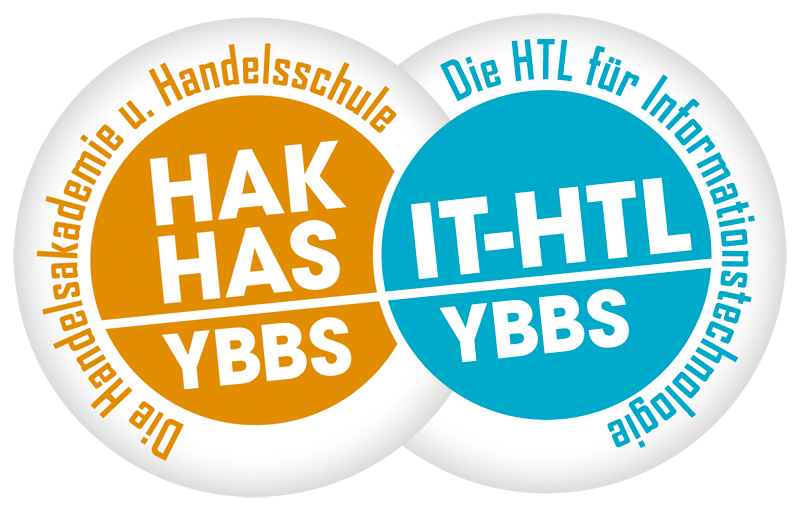
\includegraphics[width=0.5\linewidth]{images/SZ-Ybbs-Logo}
	\caption[Short Description]{Short Description}
	\label{fig:sz-ybbs-logo}
\end{figure}

\chapter{Ergebnisdokumentation}
\lfoot{Name 2}

Sample Table without label:

\begin{itemize}
	\item 	Item 1
	\item 	Item 2
\end{itemize}

Sample Math Formula: \\

$4 + 4 = ?$ \\


Text citation sample
\textcite{Vigna}. \\


\textbf{Bold Text Example}

Another text citation \textcite{OWASP},  \\

( ...  ) \\

Parencite Example \parencite{embroker}. \\

\textbf{Constructivism}

( ...  ) Third textcite \textcite{DeciRyan} \emph{Table 3}:

\begin{table} [H]
	\begin{tabular}{ |p{4cm}| p{9.0cm}| }
		\hline
		\textbf{Model}& \textbf{Characteristics}\\
		\hline
		Behaviorism & Wanted output is triggered by an appropriate input. Authoritarian model; the teacher knows what to do and shall find ways to impose his ideas on the student. \\
		Cognitivism & The learner solves given tasks on their own The teacher attends the learning process, observes, where necessary provides aid. \\
		Constructivism & Focus on personal experience. The learner is tasked with solving complex problems and have to find solutions on their own. The teacher fulfills a 	role akin to a coach. The Teacher provides aid by means of his experience and expertise in solving complex problems. \\
		\hline
	\end{tabular}
	\caption{\label{tab:learningModelComparison} Comparing Lerning Models}
\end{table}

\begin{lstlisting}
	System.console.write("Hello world");
\end{lstlisting}

( ... )

Bibliography{.}


